\chapter{Quantum Chromodynamics}
\label{chap:QCD}

The strong interaction is the fundamental force responsible for binding quarks together into hadrons. It is described by \ac{QCD} which is a gauge theory based on $SU(3)_{C}$ symmetry. One of the key features of \ac{QCD} is the phenomenon known as asymptotic freedom, namely strong force weakens at shorter distances. This property differentiates the strong force from all three other fundamental forces. A brief description of the formulation of \ac{QCD} is given in \autoref{sec:QCD}. Asymptotic freedom predicts that the strong coupling constant, denoted by $\alpha_{S}$, is small at short distances, which allows for perturbative expansion of the probability amplitude. However, the expansion parameter $\alpha_{S}$ at long distances becomes too large and the predictions are therefore no longer reliable. Techniques developed to model \ac{QCD} phenomenon in this regime are collectively known as nonperturbative-\ac{QCD}, which is discussed in \autoref{sec:npQCD}. Finally, the physics of hadron collisions is discussed in \autoref{sec:Collision}.

\section{Formulation of QCD}
\label{sec:QCD}

The theory of strong interaction began taking its current form in 1964 when the quark model was independently proposed by American physicist George Zweig~\cite{Zweig:1964ruk} and his Ph.D. advisor Murray Gell-Mann~\cite{Gell-Mann:1964ewy}. The original objective of this model was to explain the spectrum of new hadrons discovered at a rapid speed at the time. In this early version, mesons and baryons were viewed as composite objects formed by fractionally charged particles with a spin of $\frac{1}{2}$, named ``quarks'' by Gell-Mann and ``aces'' by Zweig. They came with several quantum charges and three different flavors: $u$, $d$, $s$. The strange quarks in this model had a higher mass, which explained the mass differences between different baryons and mesons.

This model was successful in explaining why protons of the same charge were bound together -- they were bound states of more fundamental particles affected by the strong interactions. However, gaps still existed in this model, most notably the tension with Fermi-Dirac statistics. It was indicated by this model that the wave function for $\mathrm{\Omega^{-}}$ (sss) should be symmetrical in the interchange of strange quarks. However, the wave function must be antisymmetric because quarks had half spins in this model. Gell-Mann and his collaborations were able to resolve this problem in the early 1970s by introducing color charges~\cite{Fritzsch:1973pi}. Under this updated framework, each flavor of quark should come with three colors, namely red, green, and blue. The wave functions of hadrons were assumed to be singlets of the gauge group $SU(3)_{C}$. For example, the wave function for $\mathrm{\Omega^{-}}$ baryon can be represented as,

\begin{equation}
(sss)\rightarrow(s_{r}s_{g}s_{b}-s_{g}s_{r}s_{b}+s_{b}s_{r}s_{g}-s_{r}s_{b}s_{g}+s_{g}s_{b}s_{r}-s_{b}s_{g}s_{r}),
\end{equation}

which restored the Fermi-Dirac statistics.  

The force mediators in this theory, known as ``gluons'', are massless vector bosons analogous to photons. They are electrically neutral but carry color charges, which enables the gluon-gluon self-interactions. The dynamics of gluon-gluon and quark-gluon interactions are described by the \ac{QCD} Lagrangian in the following form:

\begin{equation}
\mathcal{L}_{QCD}=-\frac{1}{2}\textsf{tr}G_{\mu\nu}G^{\mu\nu}+\bar{Q}(i\gamma^{\mu}D_{\mu}-m)Q,
\end{equation}

where $Q$ represents colour triplets quark fields $(Q_{r},Q_{g},Q_{b})^{T}$ of the $SU(3)_{C}$ group that run over six different flavors, $m$ corresponds to the mass of quarks. $G_{\mu\nu}$ is known as the gluon field strength tensor given by

\begin{equation}
\label{eq:G}
G_{\mu\nu}^{a}=\partial_{\mu}A_{\nu}^{a}-\partial_{\nu}A_{\mu}^{a}+g_{S}f^{abc}A_{\mu}^{b}A_{\nu}^{c},
\end{equation}

where $g_{S}$ corresponds to the strength of the gauge coupling. The strong coupling constant is also defined as $\alpha_{S}=\frac{g_{S}^2}{4\pi}$, which is analogous to the fine structure constant in \ac{QED}. $t_{a}$ are eight generators of the $SU(3)_{C}$ group, and $A^{a}_{\mu}$ represent eight gauge fields correspond to eight gluons. $f^{abc}$ is the structure constant defined by $[t^{a},t^{b}]=if^{abc}t^{c}$. $D_{\mu}$ is the $SU(3)_{C}$ gauge covariant derivative expresses as:

\begin{equation}
D_{\mu}=\partial_{\mu}-ig_{S}t_{a}A^{a}_{\mu}.
\end{equation}

The non-abelian structure of the $SU(3)_{C}$ group implies that the third term in Equation~(\ref{eq:G}) is nonzero as $SU(3)_{C}$ generators do not commute with each other. This leads to the trilinear and quartic gluon self-interactions when expanding the kinetic (first) term of the \ac{QCD} Lagrangian. Feynman diagrams for these gluon self-interactions are shown in Figure~\ref{fig:gluonself}.

\begin{figure}[tbh!]
 \begin{center}
 \begin{tabular}{cc}
 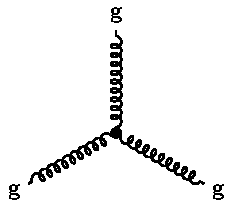
\includegraphics[width=0.45\textwidth]{figures/Part1/QCD/QCD3}&
 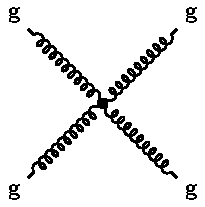
\includegraphics[width=0.4\textwidth]{figures/Part1/QCD/QCD4}\\
 \end{tabular}
 \caption{Feynman diagrams correspond to the trilinear (left) and quartic (right) gluon self-interactions.}
 \label{fig:gluonself}
 \end{center}
\end{figure}

In parallel to the development of the quark model, Feynman proposed a model to explain the behavior of deep inelastic scatterings~\cite{Feynman:1969wa}. In this model, Feynman postulated that protons are made of point-like constituents called ``partons'', and they behave like free particles at high momentum transfer. Since the de Broglie wavelength~\cite{deBroglie:1924ldk} is given by 

\begin{equation}
\lambda=\frac{h}{p}, 
\end{equation}

a high momentum transfer corresponds to a smaller wavelength and consequently better experimental resolution at the distance scale. The parton model was an immediate success as it was able to predict the short distance ``Bjorken scaling'' effects of the strong interaction at a very good precision~\cite{Bjorken:1969ja}. Despite the success at describing experimental data, the parton model was still viewed as a phenomenological approximation as Feynman provided no microscopic description of the strong interactions. It was later recognized that partons were matched to quarks, anti-quarks, and gluons within the nucleons.

Two years after Dutch physicist Gerard 't Hooft showed that non-abelian gauge theories were renormalizable~\cite{tHooft:1971akt}, major breakthrough came in 1973 when American physicists H. D. Politzer, David Gross, and Frank Wilczek~\cite{Gross:1973id,Politzer:1973fx} investigated the scale dependency of the strong coupling const $\alpha_{S}$. 't Hooft also arrived at similar results himself sometime earlier but he didn't publish his work. At one-loop precision, the $\alpha_{S}(\mu^2)$ is given by:

\begin{equation}
\label{eq:af}
\alpha_{S}(\mu^2)=\frac{\alpha_{S}(\mu_{R}^2)}{1+\beta_{0}\alpha_{S}(\mu_{R}^2)\textsf{ln}(\frac{\mu^2}{\mu_{R}^2})}
\end{equation}

where $\mu$ is the energy scale, $\mu_{R}$ is known as the renormalization scale, which corresponds to the initial energy scale at which $\alpha_{S}$ is evaluated. $\beta_{0}=(33-2n_{f})/12\pi$ is a constant that depends on the number of quark flavors that can be considered massless. Even though the strong coupling constant can not be predicted from first principles, Equation~(\ref{eq:af}) allows physicists to predict its value at an energy scale $\mu$ using its measured value at a different scale $\mu_{R}$.

Equation~(\ref{eq:af}) also reveals that when $n_{f}~<16$, the strength of the strong coupling decreases as energy increases. In other words, quarks and gluons behave like free particles at very short distances. The discovery of this property, known as ``asymptotic freedom'', by Politzer, Gross, and Wilczek brought the \ac{SM} to its current formulation. Since then it has withstood the test of numerous measurements conducted at various experiments across a wide range of energy spectrum. A summary of recent measurements of $\alpha_{S}$ is given in Figure~\ref{fig:alphaS}.

\begin{figure}[tbh!]
 \begin{center}
 \begin{tabular}{c}
 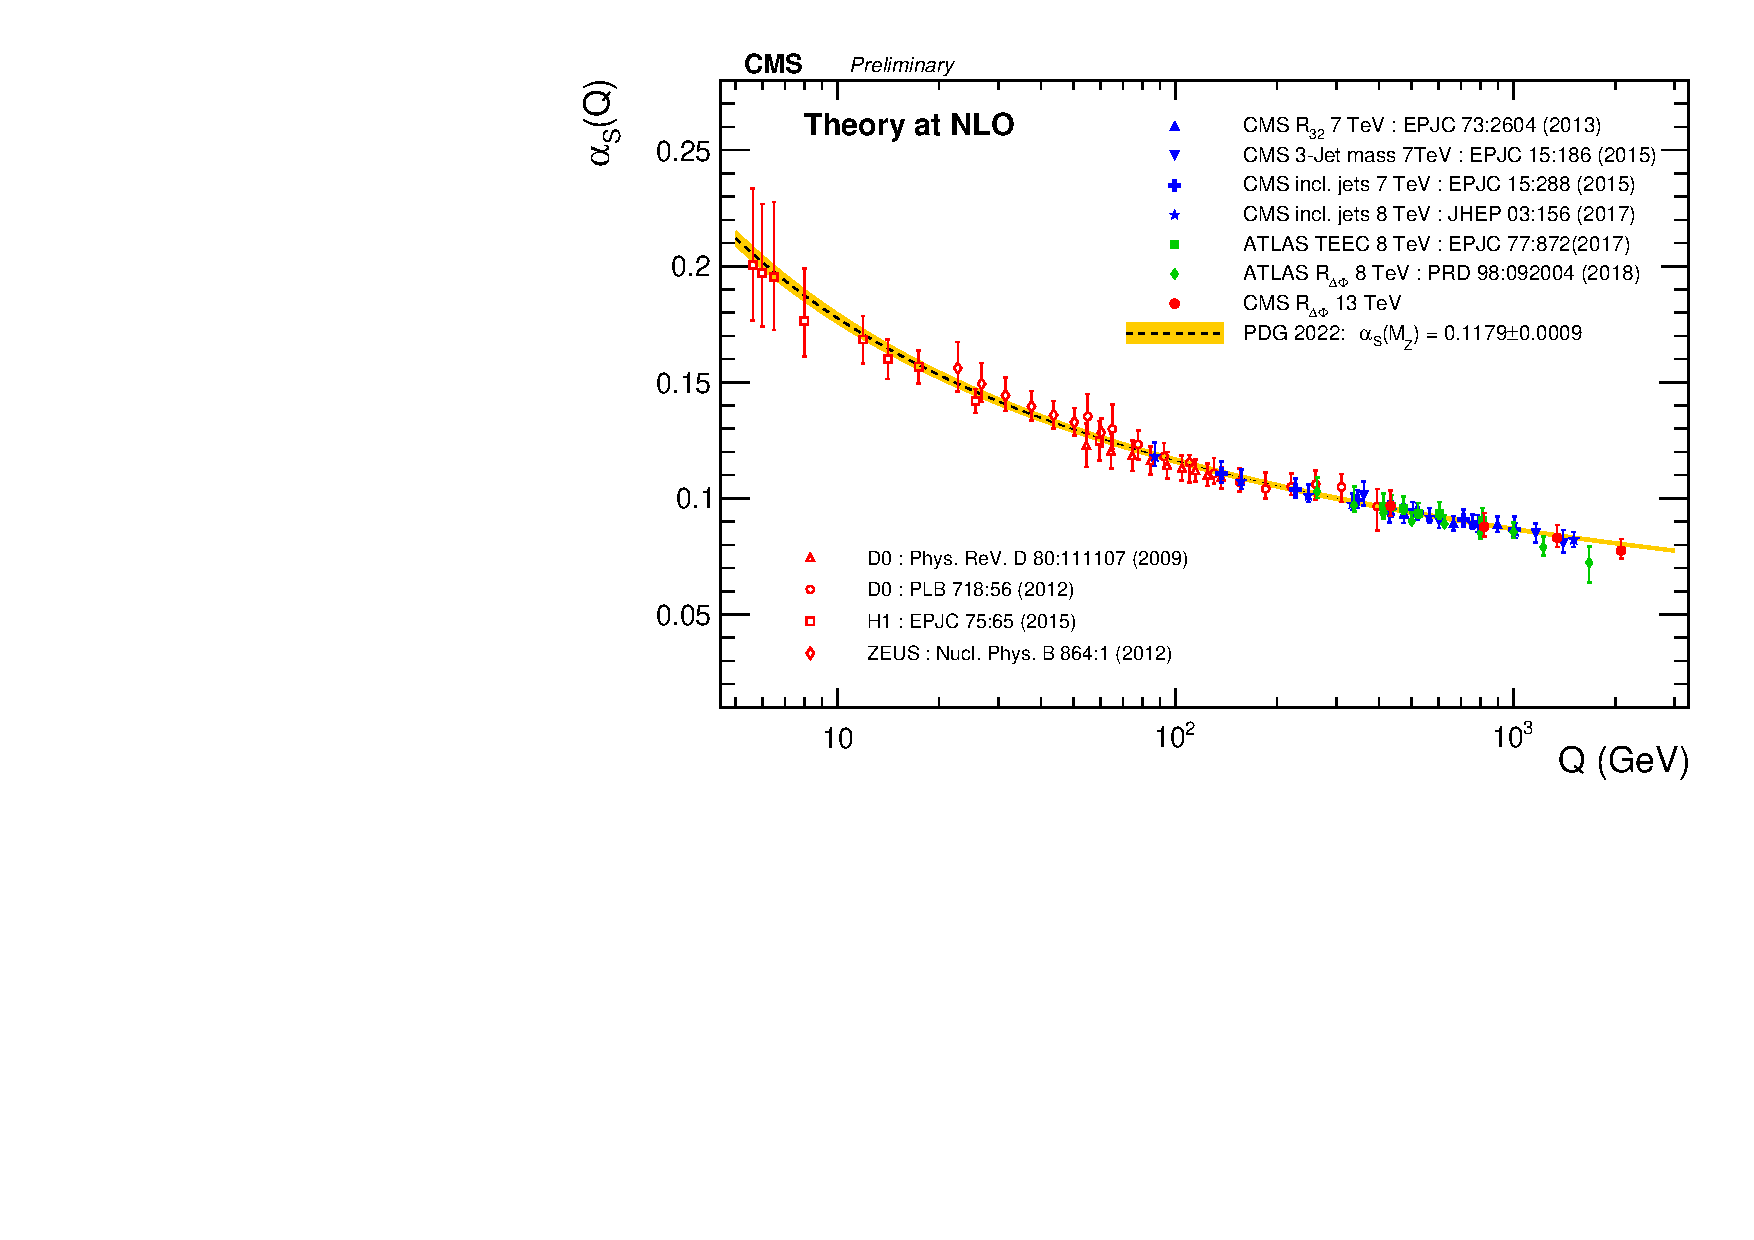
\includegraphics[width=0.8\textwidth]{figures/Part1/QCD/alphaS}
 \end{tabular}
 \caption{The strong coupling constant $\alpha_{S}$ as a function of energy scale $Q$, complied by \ac{CMS}~\cite{cms:twiki}. Measurements done by \ac{CMS}, \ac{ATLAS}, and other experiments are shown in points with uncertainty bars. Theoretical predictions based on the renormalization group equation are shown in the dashed line.}
 \label{fig:alphaS}
 \end{center}
\end{figure}

\section{Nonperturbative QCD and Factorization}
\label{sec:npQCD}

Perturbation theory is by far the best-developed tool for calculating scattering cross-sections from first principles. Despite being very successful, its predicting power becomes increasingly worse as the expansion parameter grows larger. As discussed earlier, the strong interaction grows stronger very rapidly at low energy which invalidates the perturbative expansions of parameter $\alpha_{S}$. The transition from perturbative \ac{QCD} regime to nonperturbative \ac{QCD} regime is illustrated in Figure~\ref{fig:pQCD}. The energy scales at which $\alpha_{S}$ diverges is known as $\mathrm{\Lambda}_{\textsf{QCD}}$, which is roughly $\mathcal{O}$(300 MeV)~\cite{Deur:2016tte}.

\begin{figure}[tbh!]
 \begin{center}
 \begin{tabular}{c}
 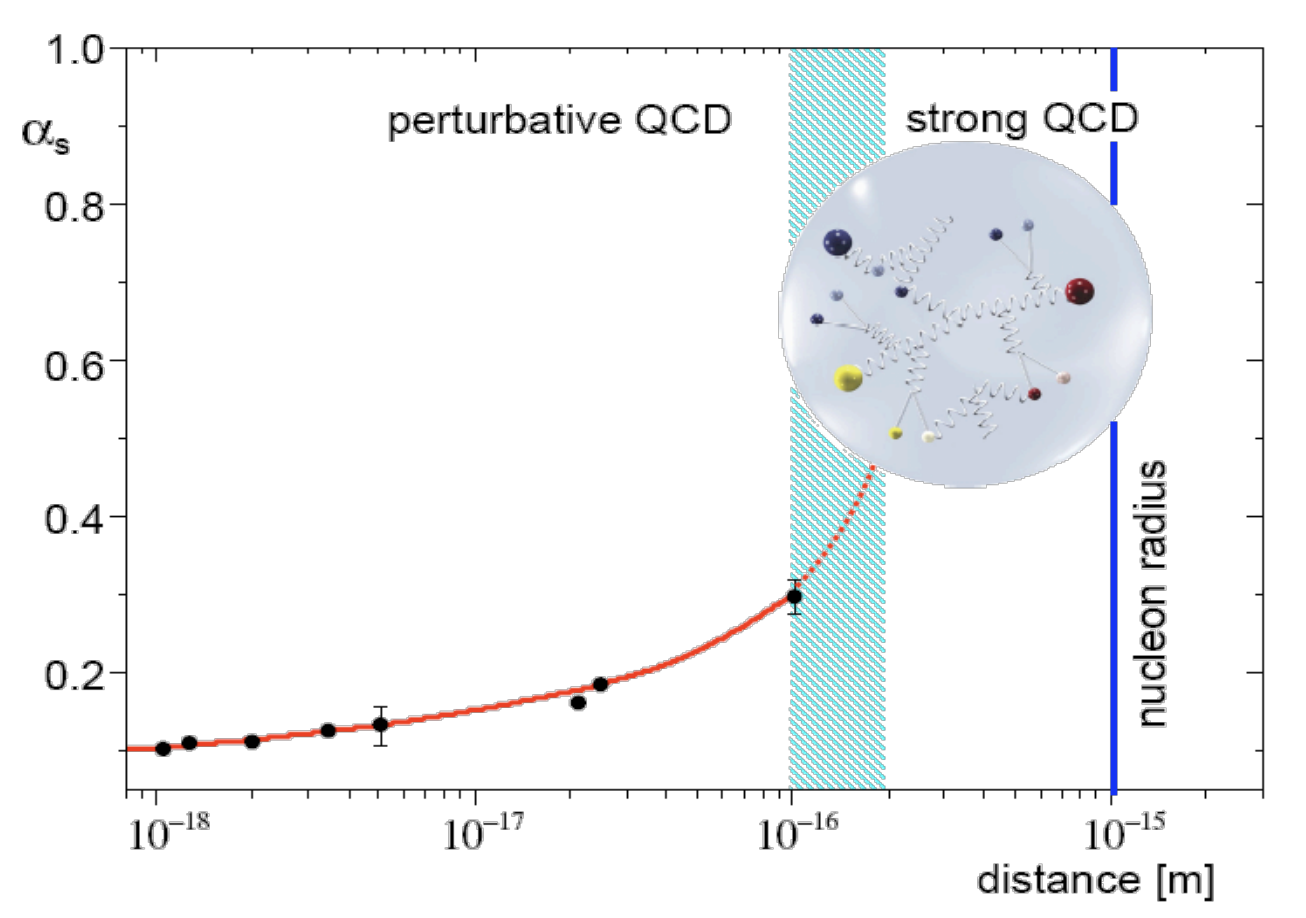
\includegraphics[width=0.7\textwidth]{figures/Part1/QCD/pQCD}
 \end{tabular}
 \caption{Illustration of the dependency of the strong coupling constant $\alpha_{S}$ on the distance scale, adapted from~\cite{Messchendorp:2013ysj}. Experimental determinations are shown in filled points while theoretical predictions are shown in the red line. The dashed blue band separates the regime where the perturbative approach is still valid from the regime where the perturbative approach is no longer valid.}
 \label{fig:pQCD}
 \end{center}
\end{figure}

The high-energy hadron collisions involve phenomena occurring on a wide range of distances or energy scales. The process that carries the highest momentum transfer in a collision event, referred to as ``hard scattering'', typically involves short-distance quark-gluon interactions where production cross-sections calculated by perturbative \ac{QCD} are still valid. It is therefore critically important to separate the hard scattering from those long-distance effects in order to apply the perturbative \ac{QCD} in any cross-section calculations. This is achieved through the so-called \ac{QCD} ``factorization theorem''~\cite{Collins:1989gx} whereby scattering cross-sections are decomposed as the product of several ``factors''. Each of these factors involves phenomena occurring on a single distance scale. An illustration of the factorization is shown in Figure~\ref{fig:factorization}.

\begin{figure}[tbh!]
 \begin{center}
 \begin{tabular}{c}
 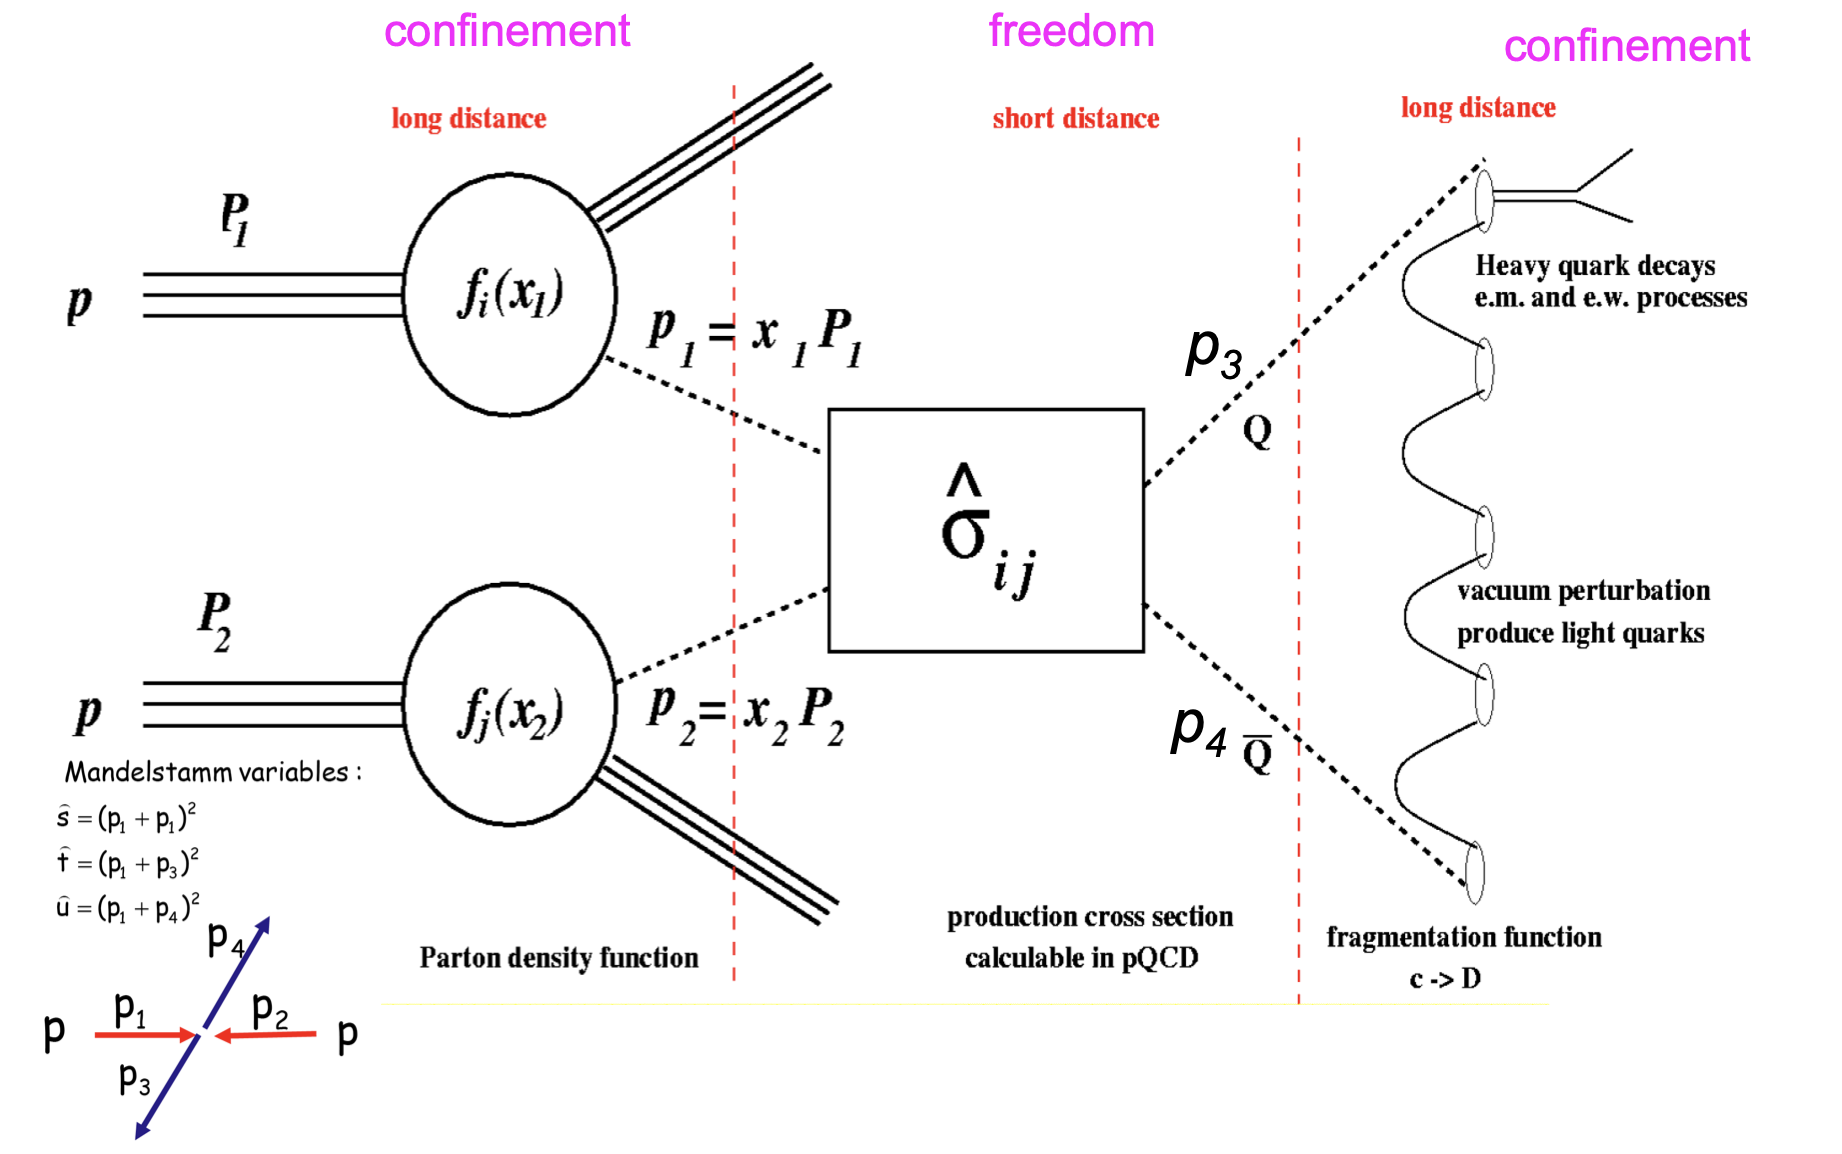
\includegraphics[width=0.9\textwidth]{figures/Part1/QCD/factorization}
 \end{tabular}
 \caption{Illustration of the physics of proton-proton collisions, adapted from~\cite{Huston:fact}. The two incoming protons are shown on the left. The \ac{PDF} characterizes the properties of the two partons that participate in a hard interaction. The short-distance physics is handled by the perturbative \ac{QCD} which is represented with the rectangular box. The outgoing partons fragment into hadrons which is described by the \ac{FF}.}
 \label{fig:factorization}
 \end{center}
\end{figure}

Protons are made of two up quarks and one down quark, known as the ``valence quarks''. Since the total mass of the three valence quarks is much smaller than the mass of a proton, most of the proton mass manifests as strong interactions within the nucleons. The mediators of these interactions -- the gluons can also spawn a pair of quark and anti-quark, forming part of the proton internal structure known as the ``proton sea''. Therefore, it is possible for strange, charm, or even bottom quarks to initiate a hard scattering, and the three-quark view of the proton is largely ineffective in the context of hadron collisions. Moreover, before the initial state of the hard scattering reveals itself, the quarks and gluons coming from different protons maintain a relatively large distance between each other, exchanging largely nonperturbative effects. This makes it virtually impossible to predict, from first principle, the structure of the proton before the hard scattering. 

A phenomenological approach, inspired by Feynman's parton model, is used to describe the proton's internal structure. Under this approach, protons are seen as streams of quarks and gluons, collectively known as partons. These partons are considered collinear with the proton movement and each carries a fraction of the total proton momentum. The probability of a specific parton $a$ that carries $x$ fraction of the proton momentum is given by the \ac{PDF} $F_{a}(x,\mu_{F}^2)$ where $\mu_{F}$ is the energy scale that defines the boundary between the short-distance and long-distance dynamics, known as the factorization scale. The cross-section for the inclusive production of a single hadron $X$ from proton-proton collisions is given by the so-called ``master formula'':

\begin{equation}
\label{eq:master}
\sigma_{pp\rightarrow X}=\sum_{a,b}\int_{0}^{1}dx_{1}dx_{2}dzF_{a}(x_{1},\mu_{F}^2)F_{b}(x_{2},\mu_{F}^2)\hat{\sigma}_{ab\rightarrow k}(\mu_{R}^2,\mu_{F}^2)D_{k\rightarrow X}(z,\mu_{F}^2).
\end{equation} 

As \acp{PDF} only describe nonperturbative effects below the energy scale $\mu_{F}$, they must be extracted by experimentalists from data~\cite{NNPDF:2014otw,NNPDF:2017mvq}. Analogous to the running of the strong coupling constant $\alpha_{S}$, the exact details of \acp{PDF} depend on the energy scale at which it is evaluated. The \acp{PDF} extracted at one energy scale can be related to the \acp{PDF} at another scale energy scale by the so-called ``DGLAP'' equation~\cite{Gribov:1971zn,Altarelli:1977zs,Dokshitzer:1977sg}, provided that $\mu_{F}\gg\mathrm{\Lam_{\textsf{QCD}}}$. A comparison of \acp{PDF} evaluated at different energy scales is shown in Figure~\ref{fig:PDF}. The solutions to the ``DGLAP'' equation are referred to as the renormalized \acp{PDF}, which can be used to describe the proton structures universally across experiments. 

\begin{figure}[tbh!]
 \begin{center}
 \begin{tabular}{c}
 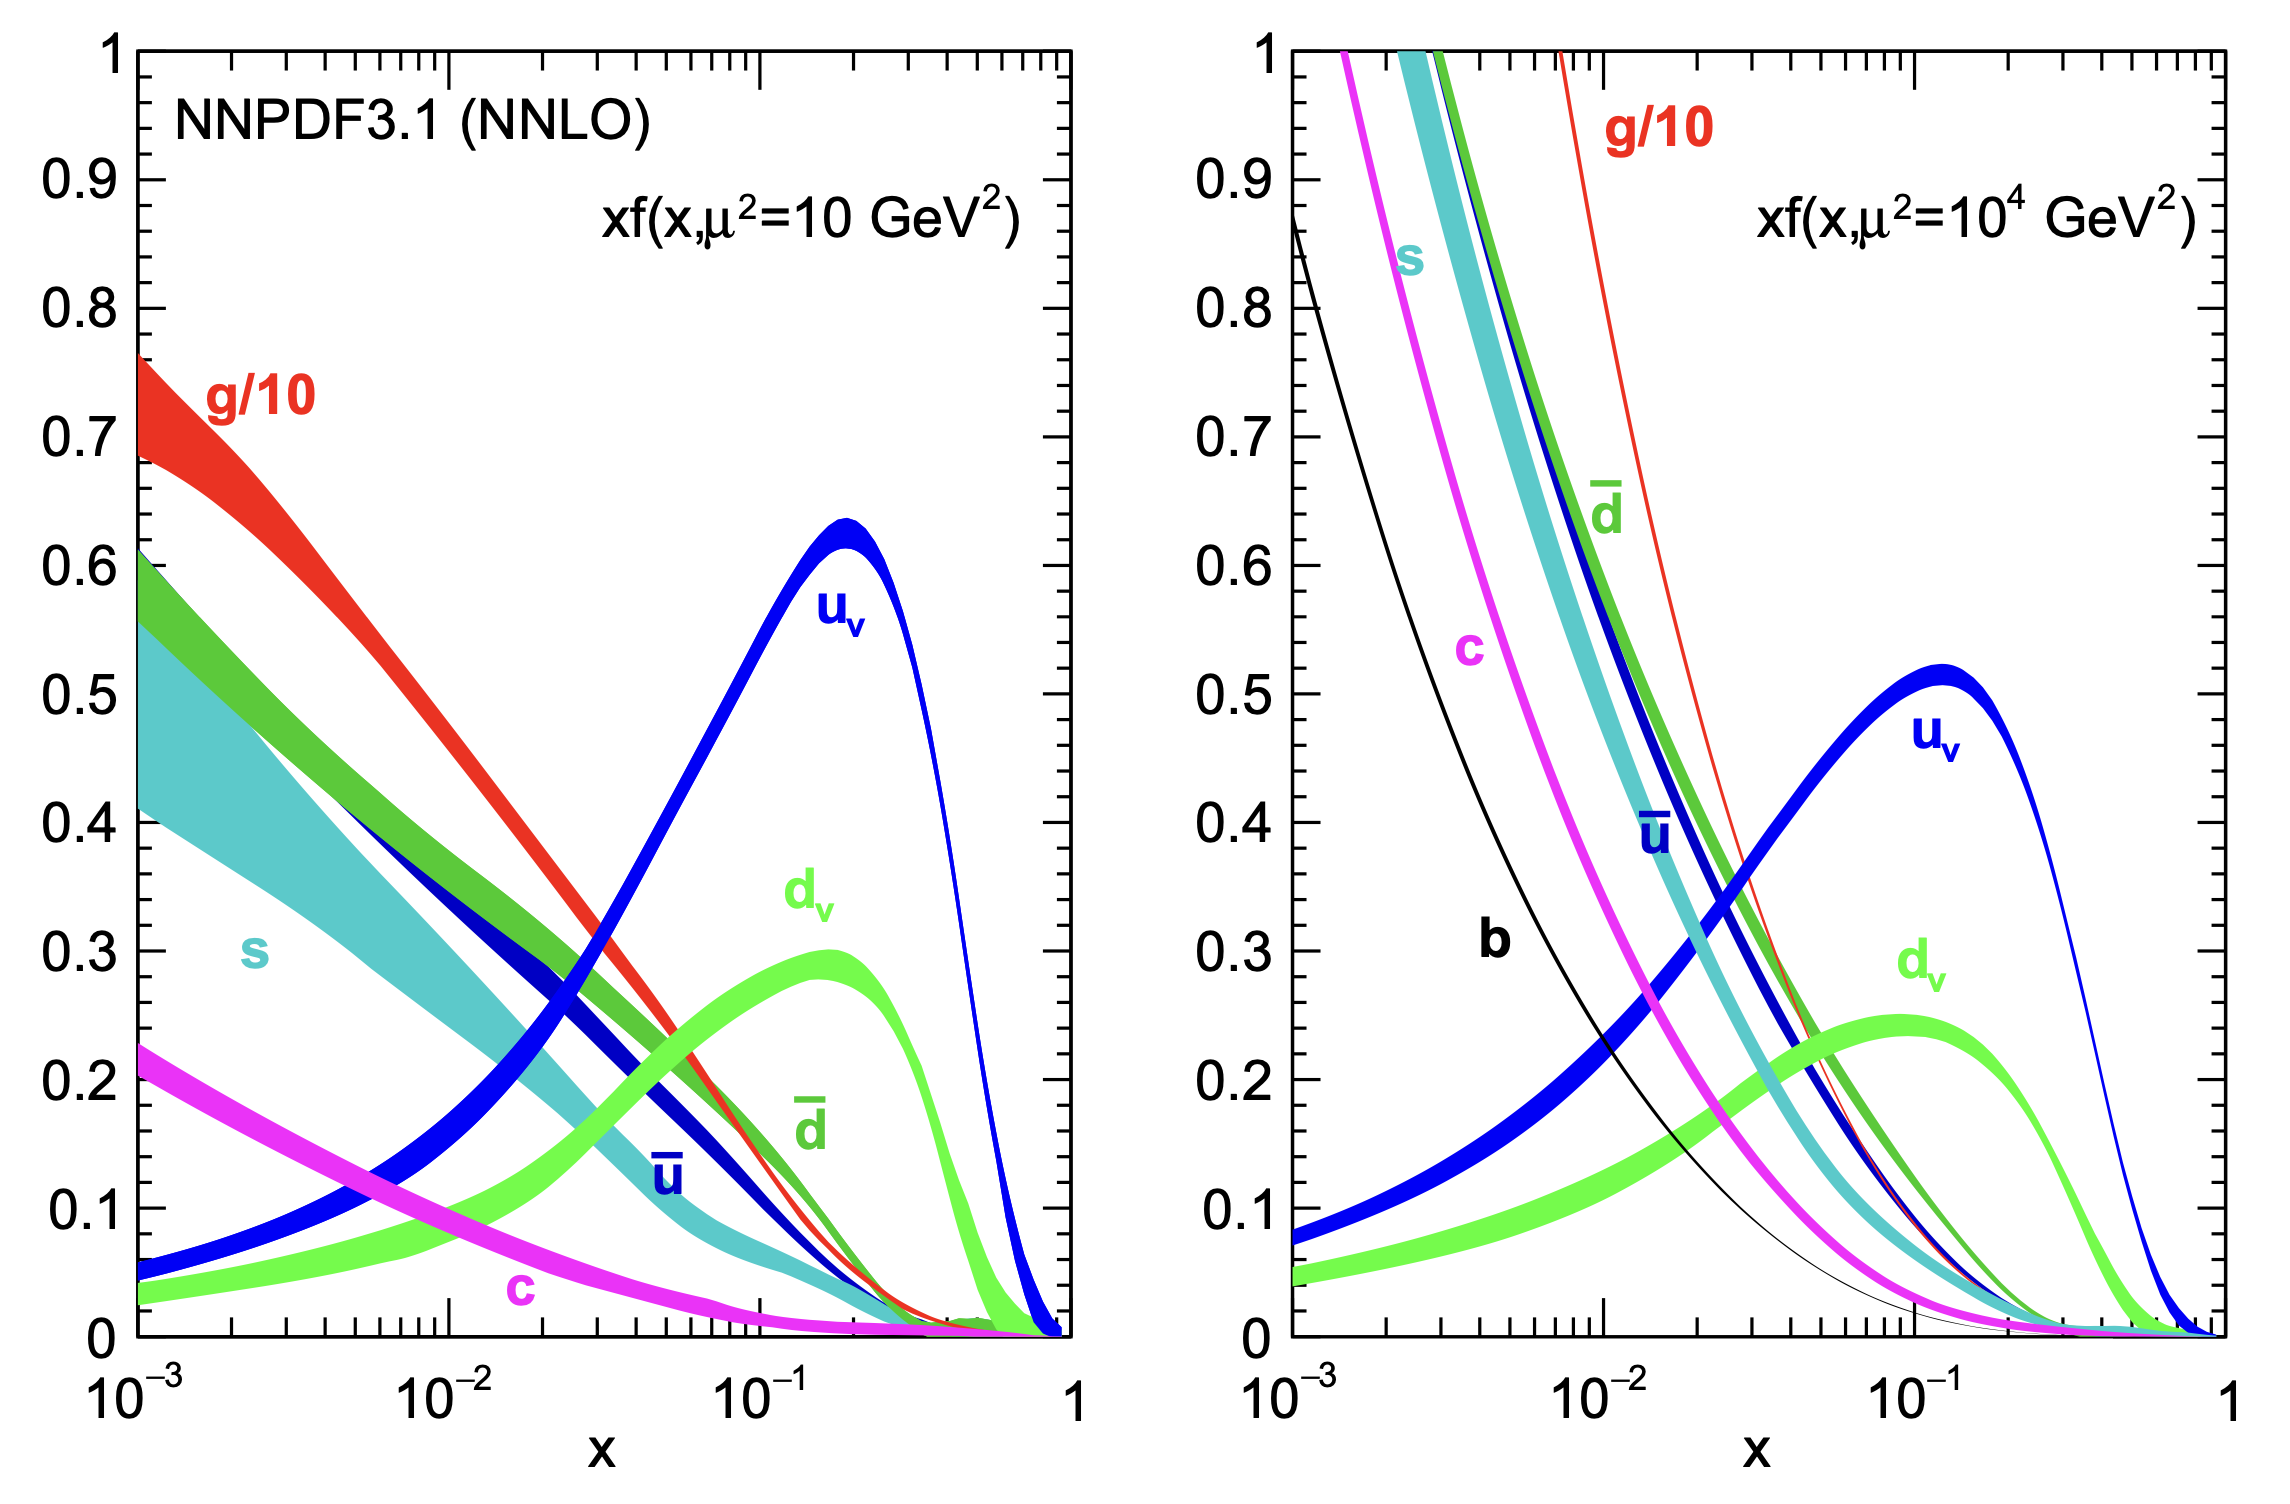
\includegraphics[width=0.8\textwidth]{figures/Part1/QCD/PDF}
 \end{tabular}
 \caption{The NNPDF3.1 \acp{PDF} multiplied by the proton momentum fraction $x$ calculated at at \ac{NNLO} accuracy in perturbation theory for $\mu^2$ = 10 $\GeV^2$ (left) and $\mu^2$ = 10$^4~\GeV^2$ (right)~\cite{NNPDF:2017mvq}. The gluon \acp{PDF} in both plots are scaled down by a factor of 10 for improved visualization.}
 \label{fig:PDF}
 \end{center}
\end{figure}

Descriptions of the short-distance physics are contained in the third factor of Equation~(\ref{eq:master}), $\hat{\sigma}_{ab\rightarrow k}$, which is the partonic cross-section for the production of partonic final states $k$ from initial partons $i$ and $j$. The initial partons $i$ and $j$ can be quarks, anti-quarks, or gluons, and all possible initial states to produce $k$ are summed over and weighted by the probabilities given by the \acp{PDF}. The partonic cross-section is given by:

\begin{equation}
\hat{\sigma}_{ab\rightarrow k}=\frac{1}{2s}\int[\prod_{i=1}^{n}\frac{d^3q_{i}}{(2\pi)^3E_{i}}][(2\pi)^4\delta^4(\sum_{i=1}^{n}q_{i}^{\mu}-(p_{a}+p_{b})^{\mu})]|\mathcal{M}_{ab\rightarrow k}(\mu_{R}^2,\mu_{F}^2)|^2,
\end{equation}

where $\frac{1}{2s}$ is the flux factor with $s$ being the squared center of mass energy of the collision. $E_{i}$, $q_{i}$ and $q_{i}^{\mu}$ are the energy, three-, and four-momentum of the parton $i$ in partonic final state $k$, respectively. $p_{a}^{\mu}$ and $p_{b}^{\mu}$ are the four momenta of the initial state partons $a$ and $b$, respectively. $\mathcal{M}_{ab\rightarrow k}(\mu_{R}^2,\mu_{F}^2)$ is the \ac{ME} that characterizes the transition rate of the partonic process $ab\rightarrow k$.

The partonic cross-section is calculated with the perturbative expansions in powers of the strong coupling constant:

\begin{equation}
\label{eq:expand}
\hat{\sigma}_{ab\rightarrow k}=\hat{\sigma}_{0}+\alpha_{s}(\mu_{R}^2)\hat{\sigma}_{1}+\alpha_{s}^{2}(\mu_{R}^2)\hat{\sigma}_{2}+...,
\end{equation}

where the linear and quadratic terms of $\alpha_{s}(\mu_{R}^2)$ are referred to as the \ac{LO} and \ac{NLO} terms, respectively. 

The last factor in Equation~(\ref{eq:master}) is referred to as the \ac{FF}~\cite{Field:1976ve} that encodes information on how color-charged partons produced in hard scatterings are turned into colorless bound states $X$ (hadrons). More specifically, the fraction $z$ of the parton momentum is transferred to the hadron $X$, and the associated probability at energy scale $\mu_{F}$ is represented by $D_{k\rightarrow X}(z,\mu_{F}^2)$. Similar to the situation of the \ac{PDF} determination, \acp{FF} constitutes in general nonperturbative components in \ac{QCD} factorization, which can not be predicted from first principle by theoretical methods. Instead, \acp{FF} are extracted from experiments and the $\mu_F$ dependency of the \ac{FF} is perturbatively calculable using the ``DGLAP'' equation.

\section{Hadron Collisions}
\label{sec:Collision}

In addition to the cross-section calculations, collider physicists often need simulated events to compare with data. Several main stages are required to simulate the full picture of a hadron collision event down to the level of stable particles before the detector response kicks in. These main stages include: hard scattering, \ac{PS}, underlying event, hadronization, and unstable particle decay.

Generation of the hard scattering events is usually done by \ac{ME} event generators, such as \MG~\cite{Alwall:2014hca} and \Pow~\cite{Frixione:2007vw}. Depending on what processes are targeted, these \ac{ME} generators determine the relevant Feynman diagrams and use \ac{MC} methods to generate initial- and final-state particles with properties such as four-momenta and spins. Each generated event is weighted by the corresponding transition rate, which is calculated numerically using the fixed-order perturbative theory. The \ac{NLO} expansions are commonly used in these perturbative calculations, which typically means one extra parton is added to the \ac{ME}.

Beyond the \ac{NLO}, it will become increasingly challenging for numerical calculations to be implemented in \ac{ME} generators. Therefore, the missing high-order terms in \ac{ME} are often approximated using a method known as the \ac{PS}. The \ac{PS} uses splitting functions~\cite{Buckley:2011ms} to characterize the emissions of soft and collinear partons by the initial-state and final-state partons. Since the emitted partons can further emit partons themselves, this process will include partons with lower and lower energy until perturbative theory breaks down, and finally produces a shower of partons. The interaction scale in \ac{PS} is considered to be perturbative. 

In addition to the hard scattering process, multiple soft parton-parton interactions exist in every collision event. These soft parton interactions, referred to as underlying event, fill events with soft partons which can then interfere with hard scattering. These interactions typically carry a low momentum transfer and thus fall into the nonperturbative \ac{QCD} regime. They are often described by data-driven phenomenological models in event generators~\cite{Sjostrand:2014zea}.

The \ac{FF} described in \autoref{sec:npQCD} does not give a detailed description of the mechanism by which partons produced in hard scatterings or heavy particle decays form the hadrons that are observed in the final state. For this reason, \acp{FF} are rarely used in \ac{MC} event generators. A more physical description would be: i) high-energy partons will first create a cascade of partons through the \ac{PS} and ii) low-energy partons that emerge from the \ac{PS} will then pick up color-matching partners to form color-neutral hadrons observed in the final state. The transition from low-energy partons to hadrons is referred to as hadronization, which is inherently an unperturbative process due to the low interaction scale near the end of the \ac{PS}. Therefore, it can only be simulated using phenomenological models such as the so-called ``Lund string'' model~\cite{Andersson:1983ia}.

Unstable hadrons produced in the hadronization process will decay sequentially, which is typically the final stage of event generation. These decays are often simulated by phenomenological models, such as the EvtGen package~\cite{Lange:2001uf}, which take input from \ac{PDG}~\cite{ParticleDataGroup:2022pth}.